\chapter{Phương pháp đề xuất}
\label{chapter:proposed}
\ifpdf
    \graphicspath{{Chapter3/Chapter3Figs/PNG/}{Chapter3/Chapter3Figs/PDF/}{Chapter3/Chapter3Figs/}}
\else
    \graphicspath{{Chapter3/Chapter3Figs/EPS/}{Chapter3/Chapter3Figs/}}
\fi

\markboth{\MakeUppercase{\thechapter. Tích hợp thông tin không gian ảnh vào chỉ mục ngược}}{\thechapter. Tích hợp thông tin không gian ảnh vào chỉ mục ngược}

Rất nhiều công trình được đưa ra để giải quyết bài toán truy vấn ảnh (mục \ref{local-features} và \ref{bag-of-words}). Phương pháp cơ bản để giải quyết bài toán là biểu diễn một hình ảnh dưới dạng mô hình Bag-of-visual-Words (BoW), sau đó xếp hạng các hình ảnh sử dụng phương pháp tf-idf và dùng chỉ mục ngược (inverted index) để tăng hiệu suất tính toán. Tuy nhiên, phương pháp trên vẫn còn bị giới hạn về độ chính xác do chưa sử dụng đến thông tin không gian ảnh. Các phương pháp được đưa ra trong những năm gần đây để giải quyết vấn đề này đã được giới thiệu trong mục \ref{spatial}.\\

Trong chương này, chúng tôi sẽ mô tả phương pháp đề xuất để tích hợp thông tin không gian ảnh vào chỉ mục ngược. Trước tiên chúng tôi sẽ nhắc lại những công trình khơi nguồn ý tưởng cho phương pháp của chúng tôi. Sau đó là phần trình bày chi tiết phương pháp đề xuất và những cải tiến nhằm nâng cao hiệu suất cho hệ thống.

\section{Chỉ mục ngược với biểu diễn Bag-of-Visual-Words}
\label{sec:inverted-index}
Như đã được giới thiệu sơ lược trọng mục 2.2.1, chỉ mục ngược (inverted index) là phương pháp phổ dùng để tối ưu hóa tốc độ truy vấn cơ sở dữ liệu bằng việc lưu trữ trước một ánh xạ từ nội dung đến vị trí trong cơ sở dữ liêu. Nói cách khác, chỉ mục ngược là một cấu trúc dữ liệu chủ yếu bao gồm 2 trường là khóa và giá trị. Mỗi khóa đại diện cho một \textit{từ}, và phần giá trị của tương ứng lưu trữ danh sách các văn bản có chứa từ đó. Vì vậy ta có thể dễ dàng lấy được danh sách tất cả các văn bản chứa từ truy vấn.

Chính vì sự thành công của các kỹ thuật tìm kiếm văn bản, chỉ mục ngược đã được mở rộng để sử dụng cho tìm kiếm ảnh trên cơ sở dữ liệu lớn. Để có thể xây dựng chỉ mục ngược cho cơ sở dữ liệu ảnh, mô hình BoW đã được sử dụng để biểu diễn hình ảnh. Quá trình xây dựng chỉ mục ngược như sau: (i) một bộ dò tìm các đặc trưng sẽ phát hiện những điểm quan trọng, sau đó một bộ mô tả sẽ trích rút trích được những đặc trưng xung quanh điểm đó; (ii) các đặc trưng được gom thành các cụm để tạo thành từ điển, mỗi cụm là một tập các đặc trưng gần giống nhau và trung tâm của mỗi cụm là một \textit{từ trực quan} (visual word), mỗi từ trực quan sẽ được gán một mã số khác nhau; (iii) Trường giá trị trong tệp chỉ mục ngược sẽ lưu trữ danh sách các hình ảnh có chứa các từ trực quan tương ứng. Quá trình tạo tập chỉ mục ngược (inverted file) được minh họa trong hình \ref{FigInvertedFile}.

\begin{figure}[!htbp]
  \begin{center}
    \leavevmode
    \ifpdf
      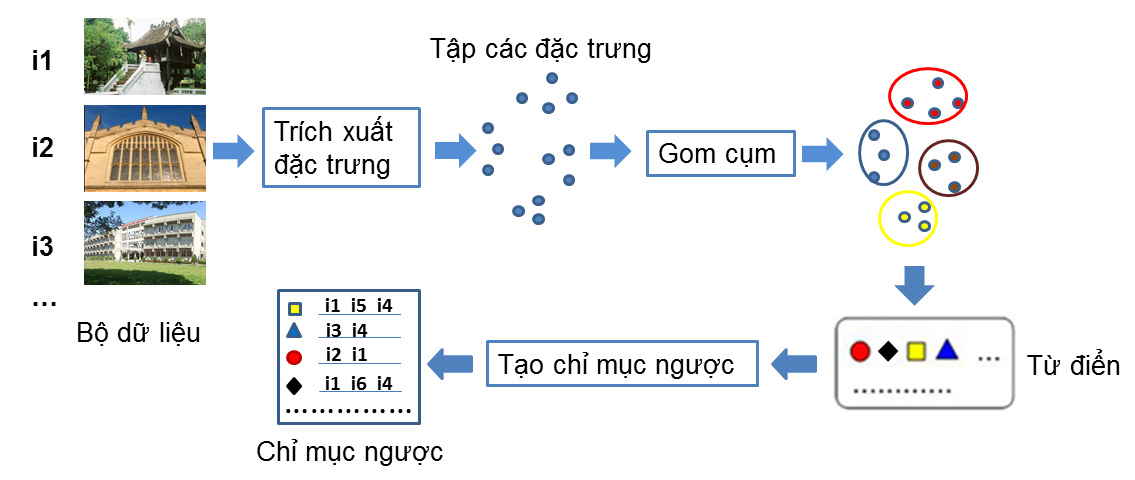
\includegraphics[scale=0.51]{invertedFile}
    \else
      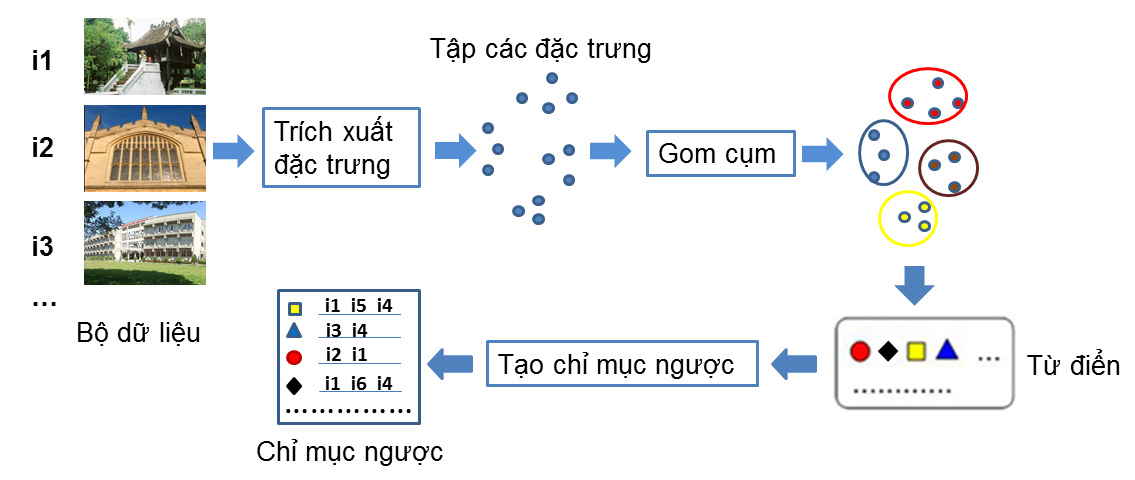
\includegraphics[scale=0.51]{invertedFile}
    \fi
    \caption[Quá trình tạo tập chỉ mục ngược]{Quá trình tạo tập chỉ mục ngược (inverted index file).}
    \label{FigInvertedFile}
  \end{center}
\end{figure}

Trong quá trình truy vấn, các đặc trưng sẽ được rút trích từ hình ảnh truy vấn, sau đó từ các đặc trưng ta sẽ lấy được các từ trực quan bằng cách sử dụng từ điển sau đó tra cứu trong tập chỉ mục ngược để lấy được các hình ảnh ứng viên. Những hình ảnh nào có số lượng từ trực quan trùng với các từ trong hình ảnh truy vấn càng nhiều thì sẽ càng được xếp hạng cao hơn trong danh sách kết quả truy vấn trả về. Kỹ thuật này được gọi là \textit{bầu chọn} (voting).

Bên cạnh kỹ thuật bầu chọn, để nâng cao độ chính xác của kết quả trả về, người ta có thể thêm một bước tái xếp hạng danh sách kết quả bằng cách tính khoảng cách trong không gian đặc trưng giữa hình ảnh truy vấn và các hình ảnh ứng viên sử dụng biểu diễn BoW của chúng. Tuy nhiên, chi phí tính toán của quá trình này rất cao dẫn đến thời gian thực hiện truy vấn tăng đáng kể.\\

Trong thí nghiệm được trình bày ở Chương 4, chúng tôi sẽ so sánh cả hai phương pháp bầu chọn và tái xếp hạng với phương pháp được đề xuất.\\

\section{Tích hợp thông tin không gian ảnh vào chỉ mục ngược}
\label{sec:intergrated}
Phương pháp chúng tôi đề xuất nhằm tích hợp thông tin không gian ảnh vào chỉ mục ngược được bắt nguồn từ ý tưởng của một công trình nghiên cứu của Lazebnik và các đồng nghiệp \cite{lazebnik2006beyond}. Trong công trình đó, thay vì sử dụng một biểu đồ (histogram) chung  của các từ trực quan để biểu diễn một hình ảnh thì họ chia hình ảnh thành các nhiều phần sử dụng lưới ô vuông phân cấp (hay còn được gọi là không gian phân cấp - spatial pyramid). Một lưới ô vuông tại cấp \textit{l} sẽ chia hình ảnh thành $2^l \times 2^l$ ô với kích cỡ như nhau. Do đó, số ô vuông trên lưới ở cấp 0 là $1 \times 1$; cấp 1 là $2 \times 2$. Nếu cấp \textit{l} càng cao thì lưới ô vuông sẽ càng dày đặc hơn. Nếu coi mỗi ô của hình ảnh được chia bởi lưới ô vuông phân cấp là một hình ảnh độc lập, dựa trên mô hình BoW ta sẽ tính được các biểu đồ độc lập. Chính vì mức độ chia tiết của các biểu đồ khác nhau nên chúng sẽ được đánh trọng số khác rồi rồi được ghép nối với nhau để tạo thành một vector đặc trưng biểu diễn cho hình ảnh. Bằng cách biểu diễn như vậy, các hình ảnh có sự phân bố các từ tương tự nhau sẽ được biễu diễn bằng những biểu đồ ghép nối gần giống nhau.

Dựa trên ý tưởng của nghiên cứu trên, chúng tôi đề xuất sử dụng không gian phân cấp để tăng cường mức độ bầu chọn và lập chỉ mục của kỹ thuật đánh chỉ mục ngược căn bản. Ý tưởng được chúng tôi đưa ra là chia hình ảnh thành nhiều ô sử dụng không gian phân cấp và giới hạn ở một cấp xác định. Sau đó các từ trực quan sẽ được đánh số tương ứng với các ô chúng rơi vào. Ta sẽ duyệt qua tất cả các ô ở tất cả các cấp khác nhau để thực hiện việc bầu chọn. Do đó, nếu hai hình ảnh chứa các từ trực quan giống nhau trong cùng một ô sẽ nhận được nhiều lượt bầu chọn hơn so với hai hình ảnh có các từ trực quan giống nhau nhưng lại nằm rải rác ở các ô khác nhau. Các lượt bầu chọn sẽ được đánh trọng số tùy theo từng cấp. Nếu cấp càng cao hay diện tích của mỗi ô càng hẹp thì trọng số của lượt bầu chọn càng cao. Trọng số tại cấp \textit{l} sẽ là $\frac{1}{2^{L-l}}$.

Một trong những điểm đặc biệt của phương pháp đề xuất là chúng tôi sử dụng đa chỉ mục ngược. Tức là chia thành nhiều tập chỉ mục ngược khác nhau nhưng các tập vẫn giữ được cấu trúc căn bản của chỉ mục ngược. Mỗi tập sẽ dùng để lưu trữ chỉ muc cho một ô trên không gian phân cấp. Nếu cấp độ cao nhất của không gian phân cấp là \textit{L} thì tổng số lượng tập chỉ mục ngược sẽ là $\frac{1}{3}(4^{L+1} - 1)$ và mỗi cấp độ sẽ có $2^l \times 2^l$ tập chỉ mục ngược với $0 \leq l \leq L$. Hình \ref{FigBasicIdea} mô tả khái quát cho phương pháp được đề xuất.

\begin{figure}[!htbp]
  \begin{center}
    \leavevmode
    \ifpdf
      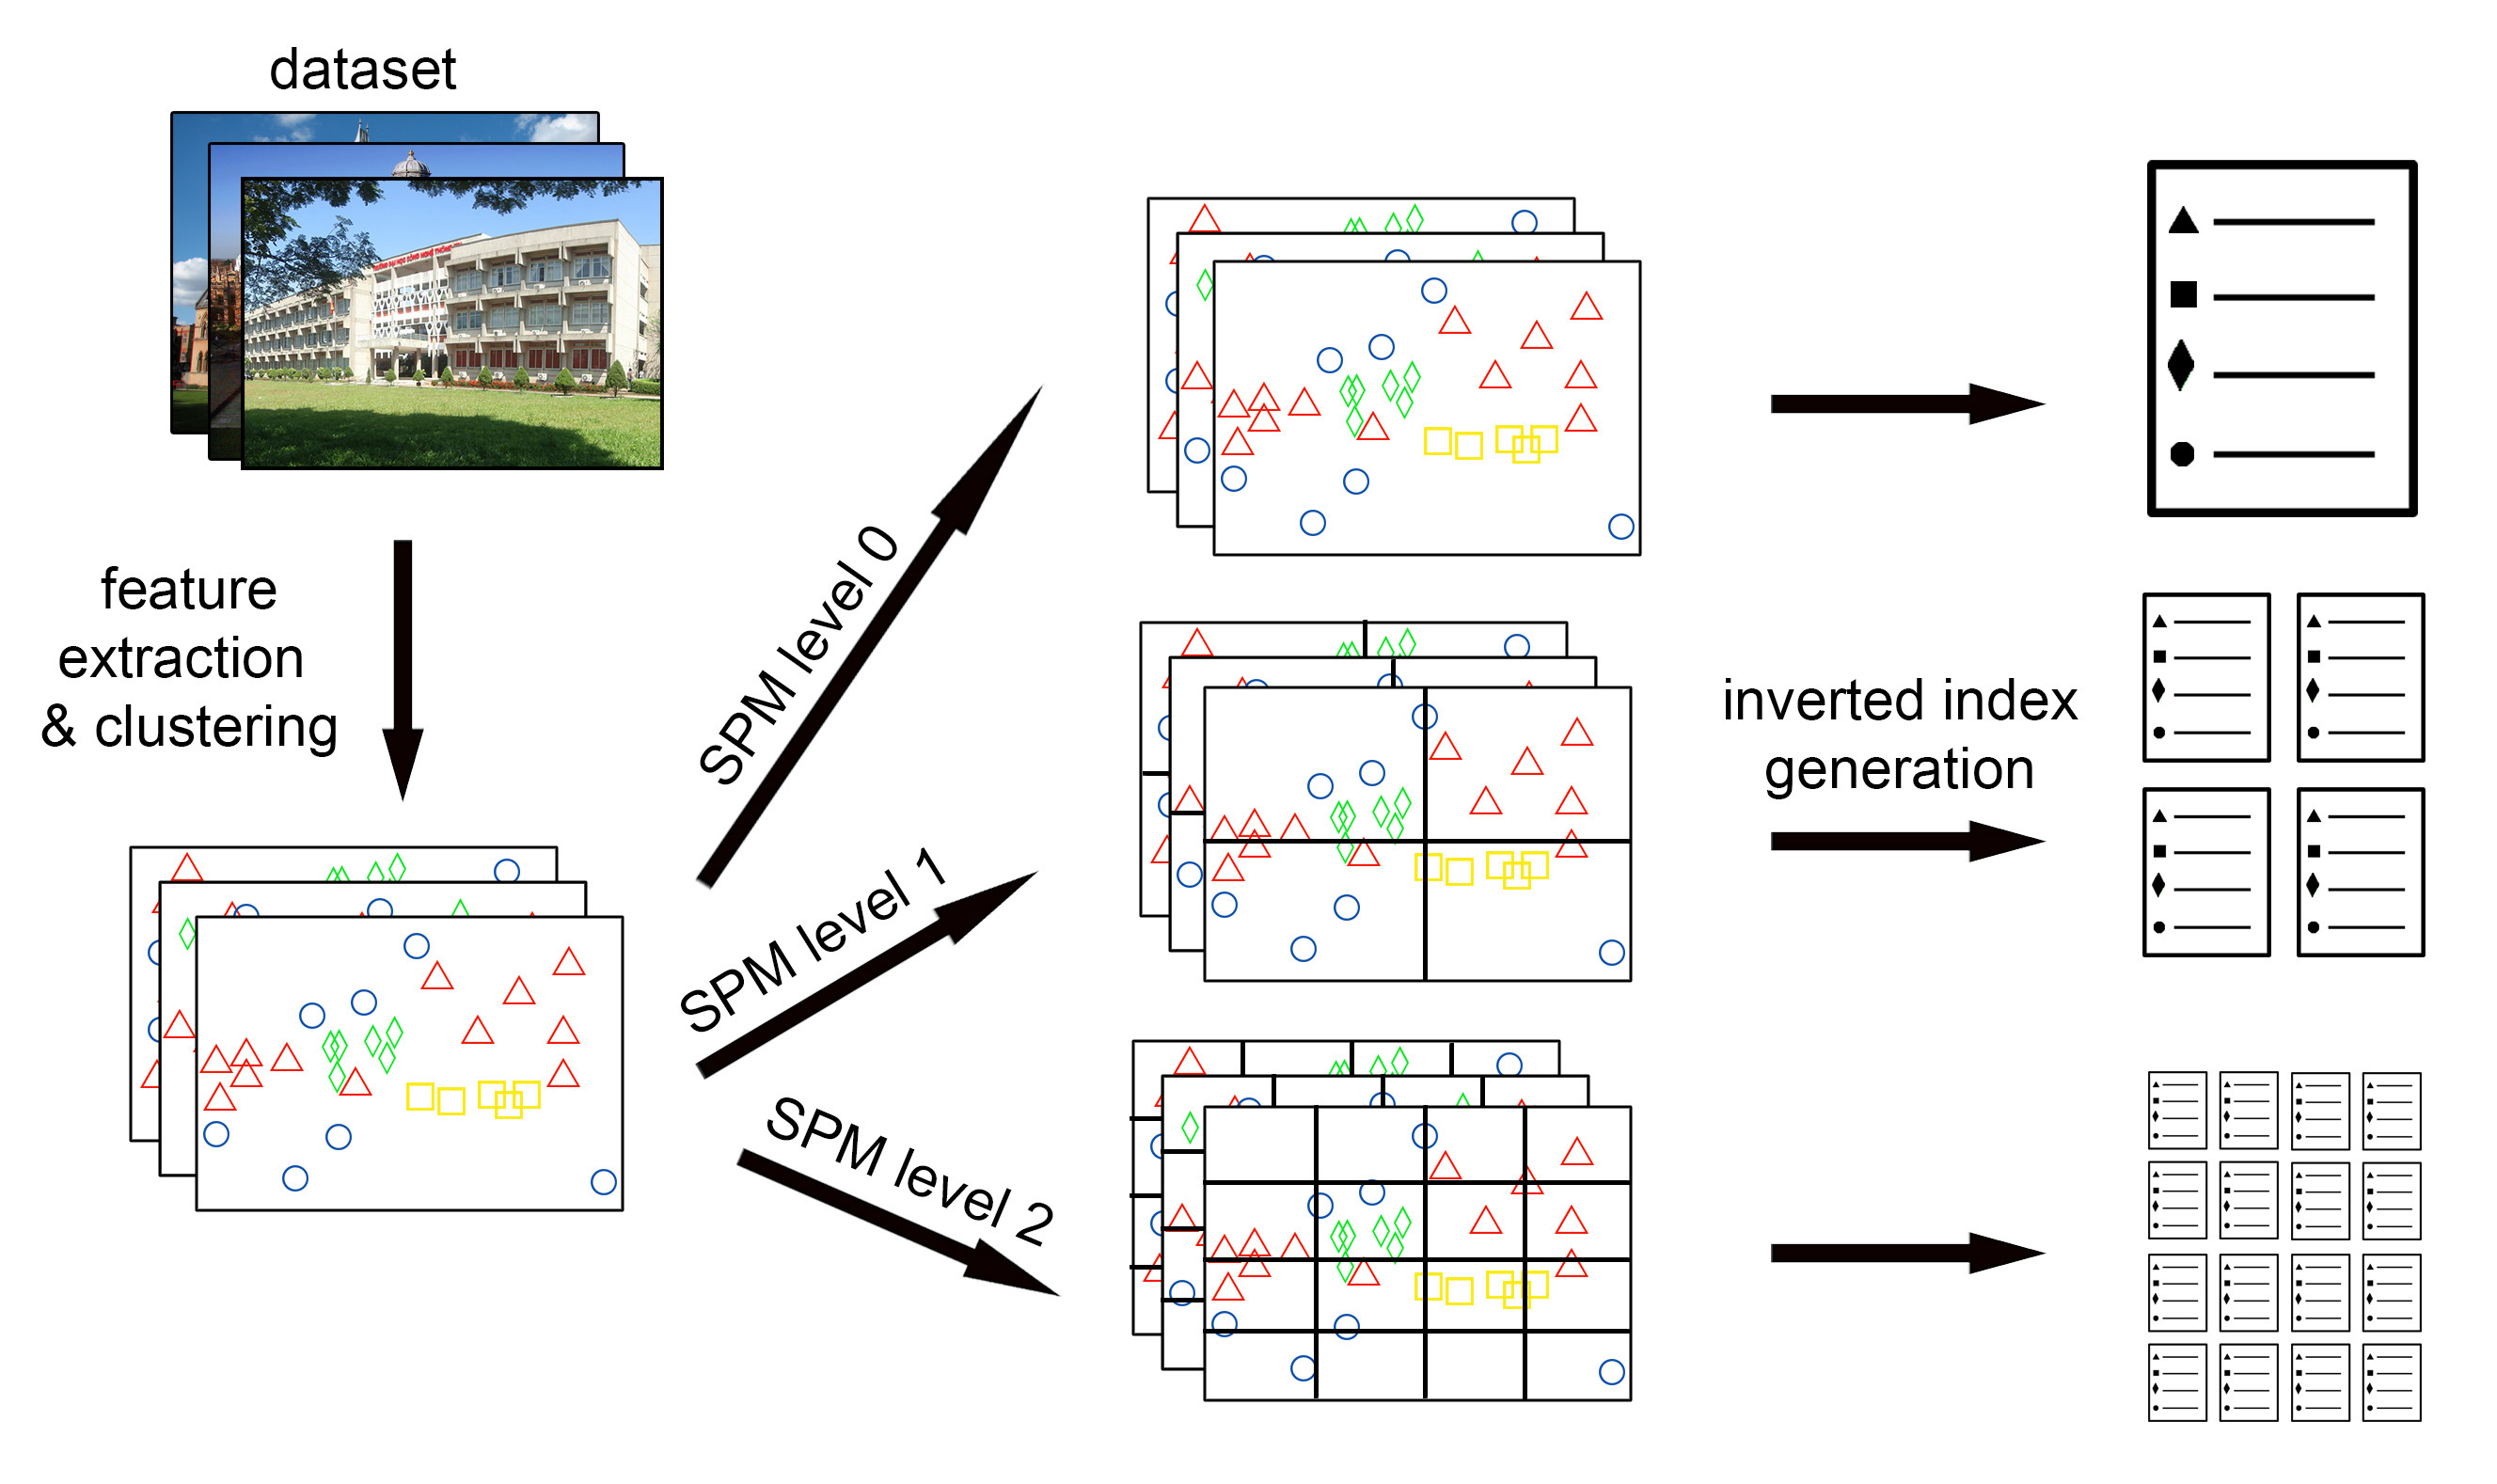
\includegraphics[scale=0.15]{basicIdea}
    \else
      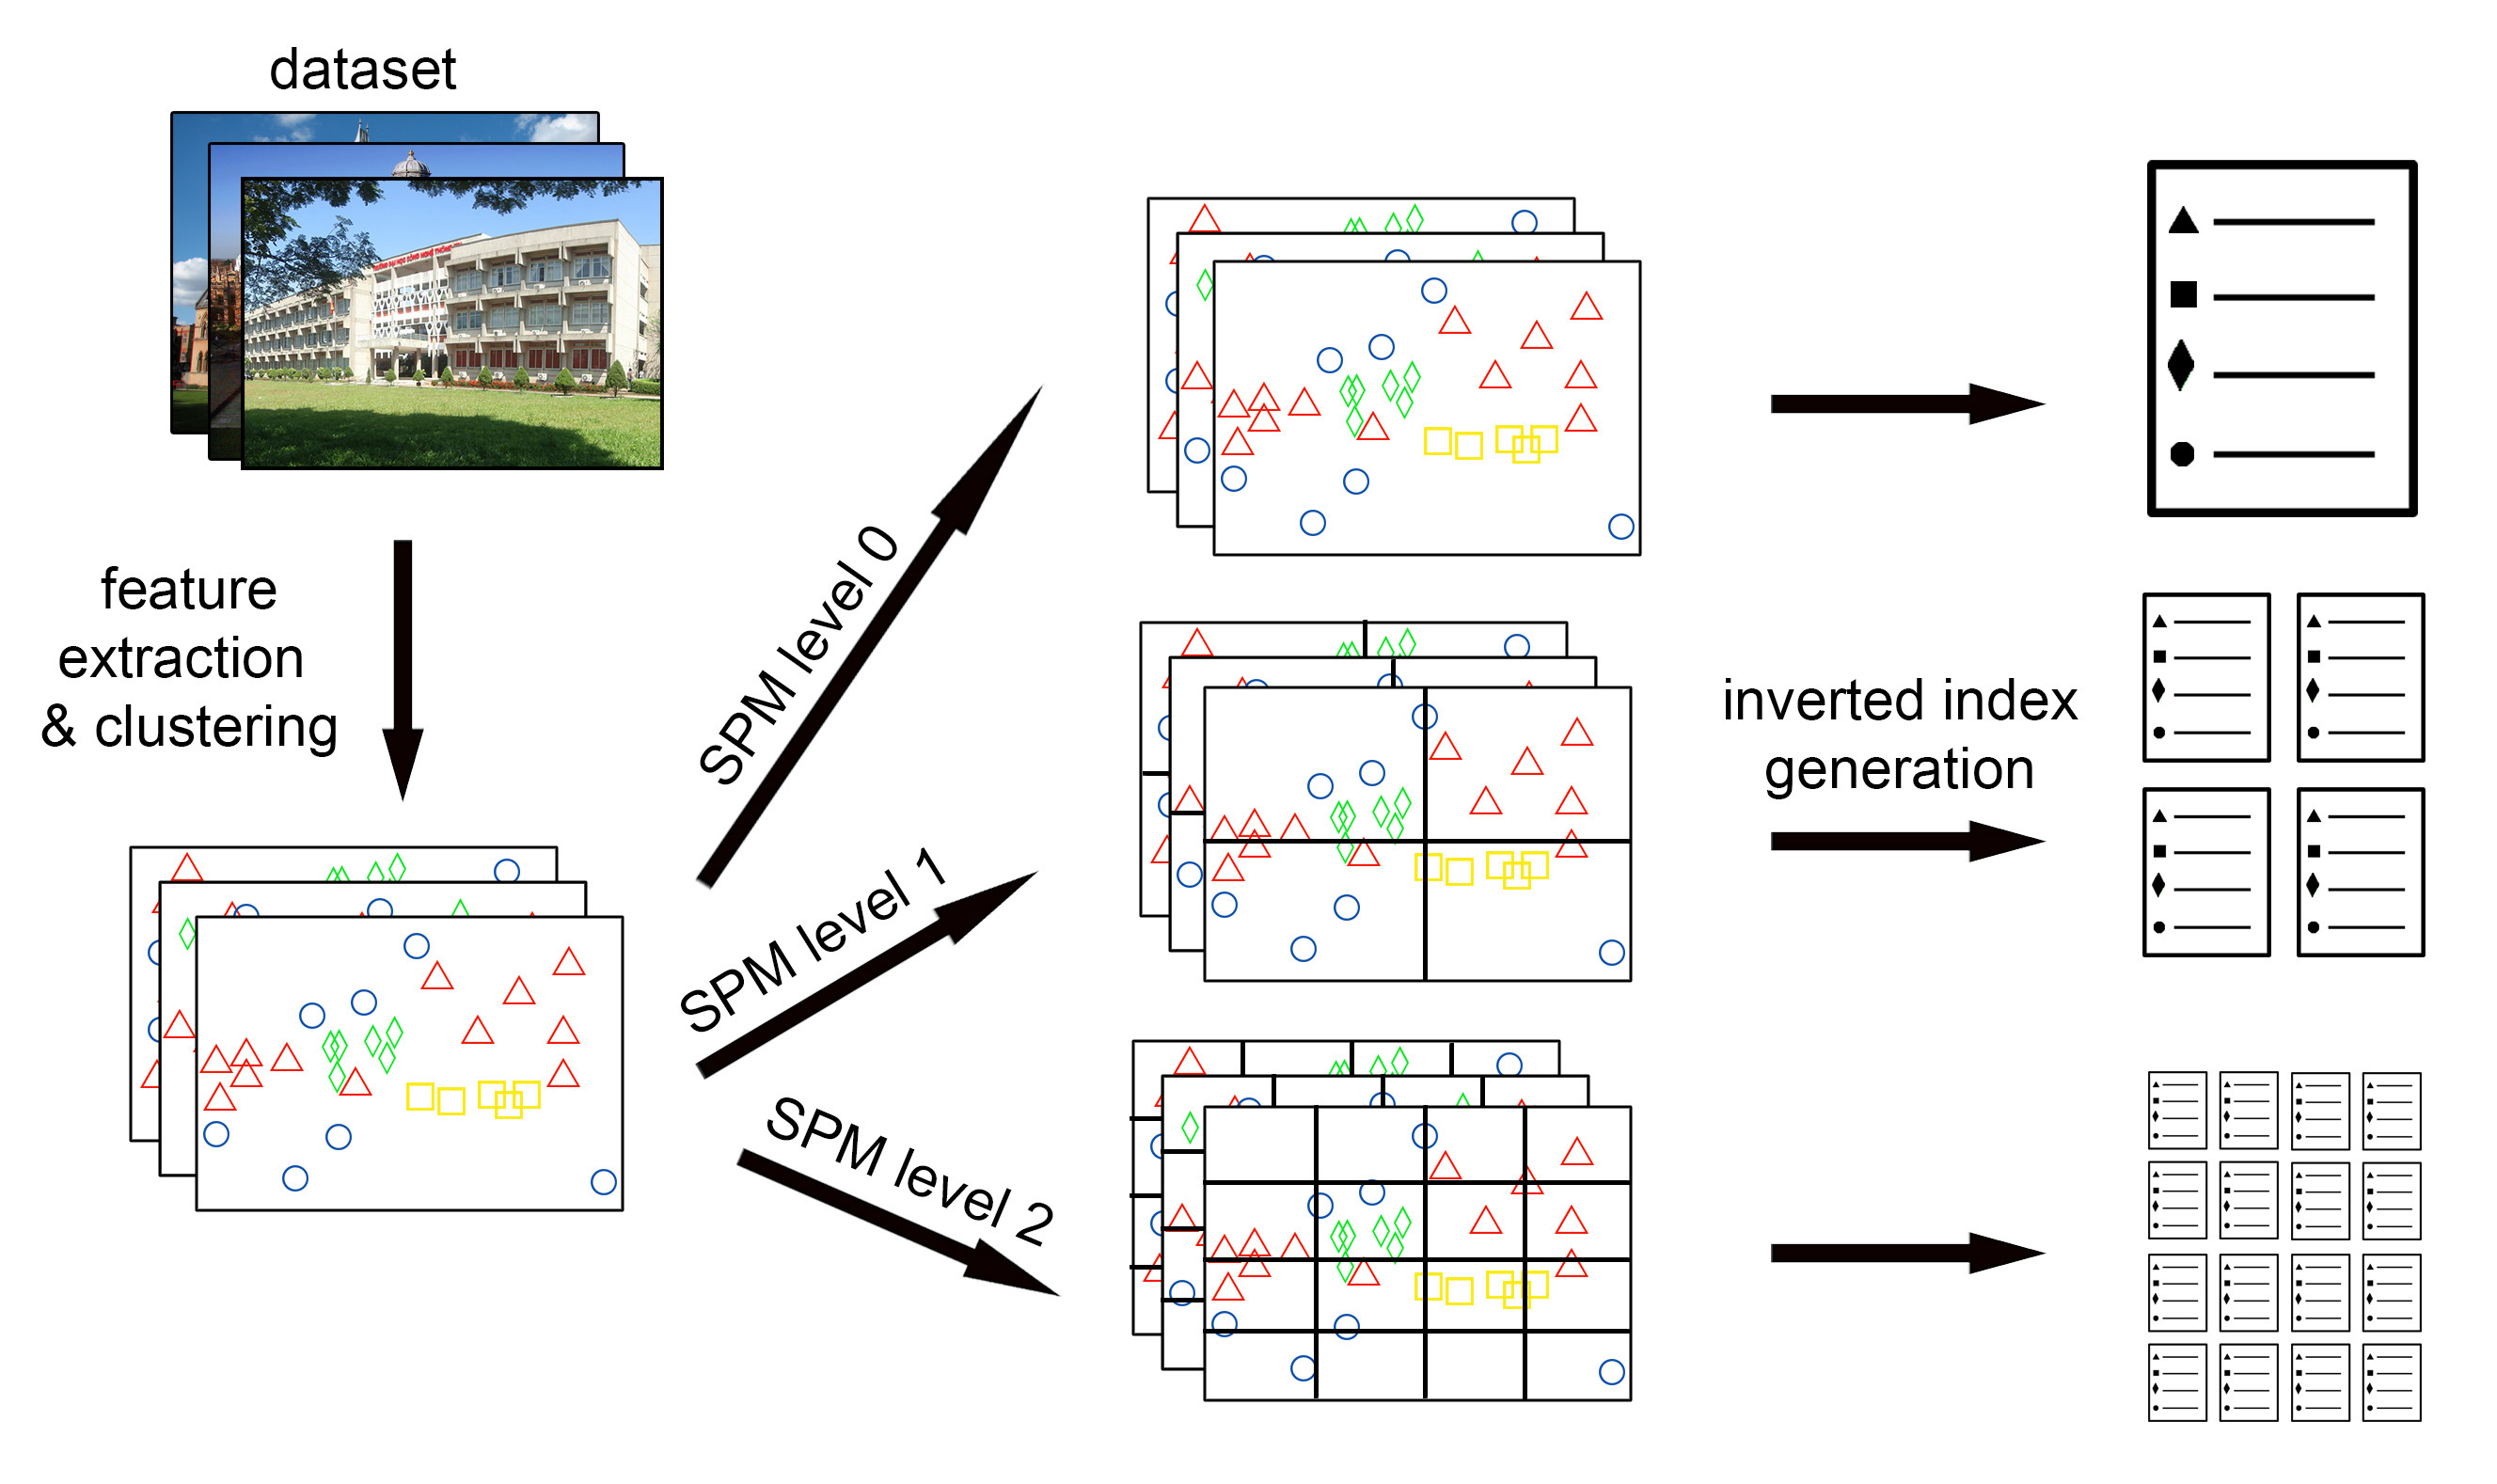
\includegraphics[scale=0.15]{basicIdea}
    \fi
    \caption[Khái quát về phương pháp đề xuất]{Khái quát về phương pháp đề xuất.}
    \label{FigBasicIdea}
  \end{center}
\end{figure}

Khi thực hiện quá trình rút trích các đặc trưng cho tất cả các hình trong cơ sở dữ liệu, thông tin không gian của các đặc trưng đó sẽ được lưu trữ lại. Sau đó các bộ mô tả (descriptors) của đặc trưng (ví dụ như key points) sẽ được lượng tử hóa để tạo thành một bảng từ vựng của các từ trực quan (từ điển). Mỗi hình ảnh sẽ chứa một tập các từ trực quan. Tiếp đó ta sẽ sử dụng không gian phân cấp để chia tất cả các hình ảnh thành các ô nhỏ với "độ mịn" tăng dần dựa trên cấp được định nghĩa. Lúc này, thông tin không gian của các đặc trưng đã được lưu trước đó sẽ được sử dụng để xác định xem từ đó có thuộc ô đang xét hay không. Tất cả các từ được tìm thấy trong mỗi ô sẽ được thu thập lại. Tiếp theo, tập hợp của các từ được tìm thấy trong mỗi ô của các hình ảnh sẽ được dùng để sinh ra một tập chỉ mục ngược tương ứng với ô đó. Số lượng tập chỉ mục ngược được sinh ra bằng với tổng số ô của không gian phân cấp.

Trong quá trình truy vấn, các đặc trưng cũng được rút trích từ hình ảnh truy vấn. Sau đó chúng được đưa vào từ điển để lấy được các từ trực quan tương ứng. Dựa vào vị trí của các từ này, ta có thể xác định được chúng thuộc ô nào tại mỗi cấp của mô hình không gian phân cấp. Từ đó ta có thể có thể truy xuất ngay lập tức tới tập chỉ mục ngược tương ứng với mỗi ô để lấy và xếp hạng danh sách hình ảnh ứng viên một cách đồng thời. Ta xếp hạng hình ảnh bằng phương pháp bầu chọn nên việc bầu chọn diễn ra trong mỗi lần truy xuất tập chỉ mục ngược, do đó danh sách đếm số lượt bầu chọn sẽ được cập nhật liên tục trong suốt quá trình truy xuất các tập chỉ mục ngược. Khi quá trình bầu chọn kết thúc, ta sẽ tổng hợp toàn bộ số lượt bầu chọn cho từng hình rồi xếp hạng các hình theo số lượt bầu chọn. Toàn bộ quá trình truy vấn của phương pháp đề xuất được minh họa trong Hình \ref{FigQueryProcess}.

\begin{figure}[!htbp]
  \begin{center}
    \leavevmode
    \ifpdf
      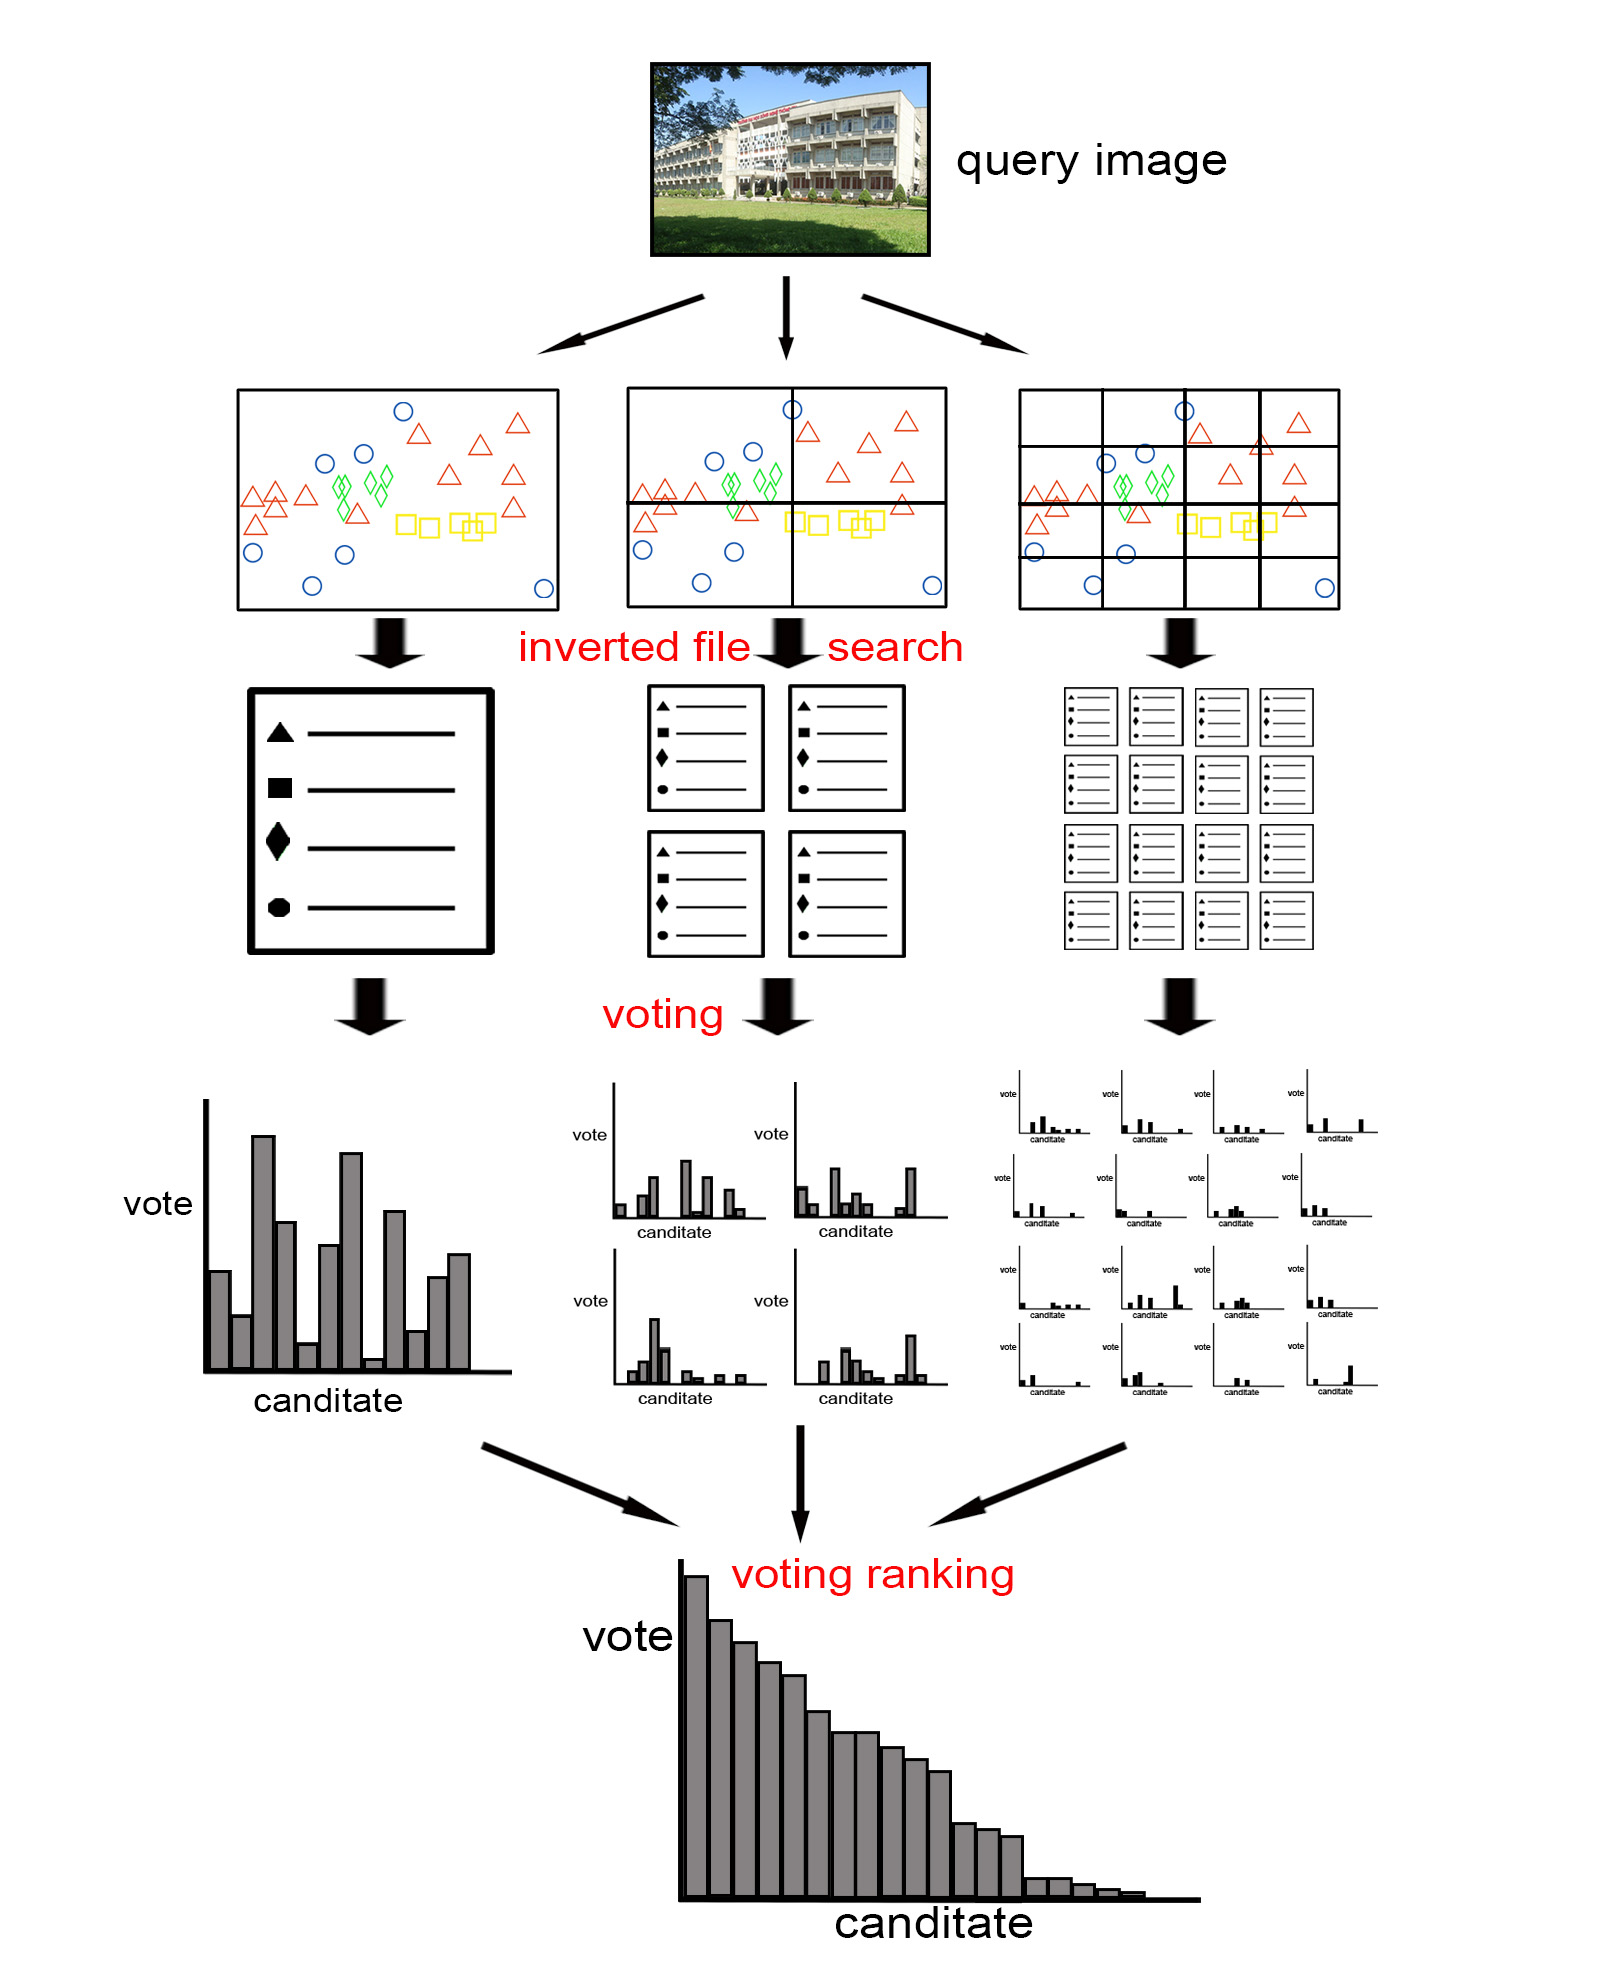
\includegraphics[scale=0.25]{queryProcess}
    \else
      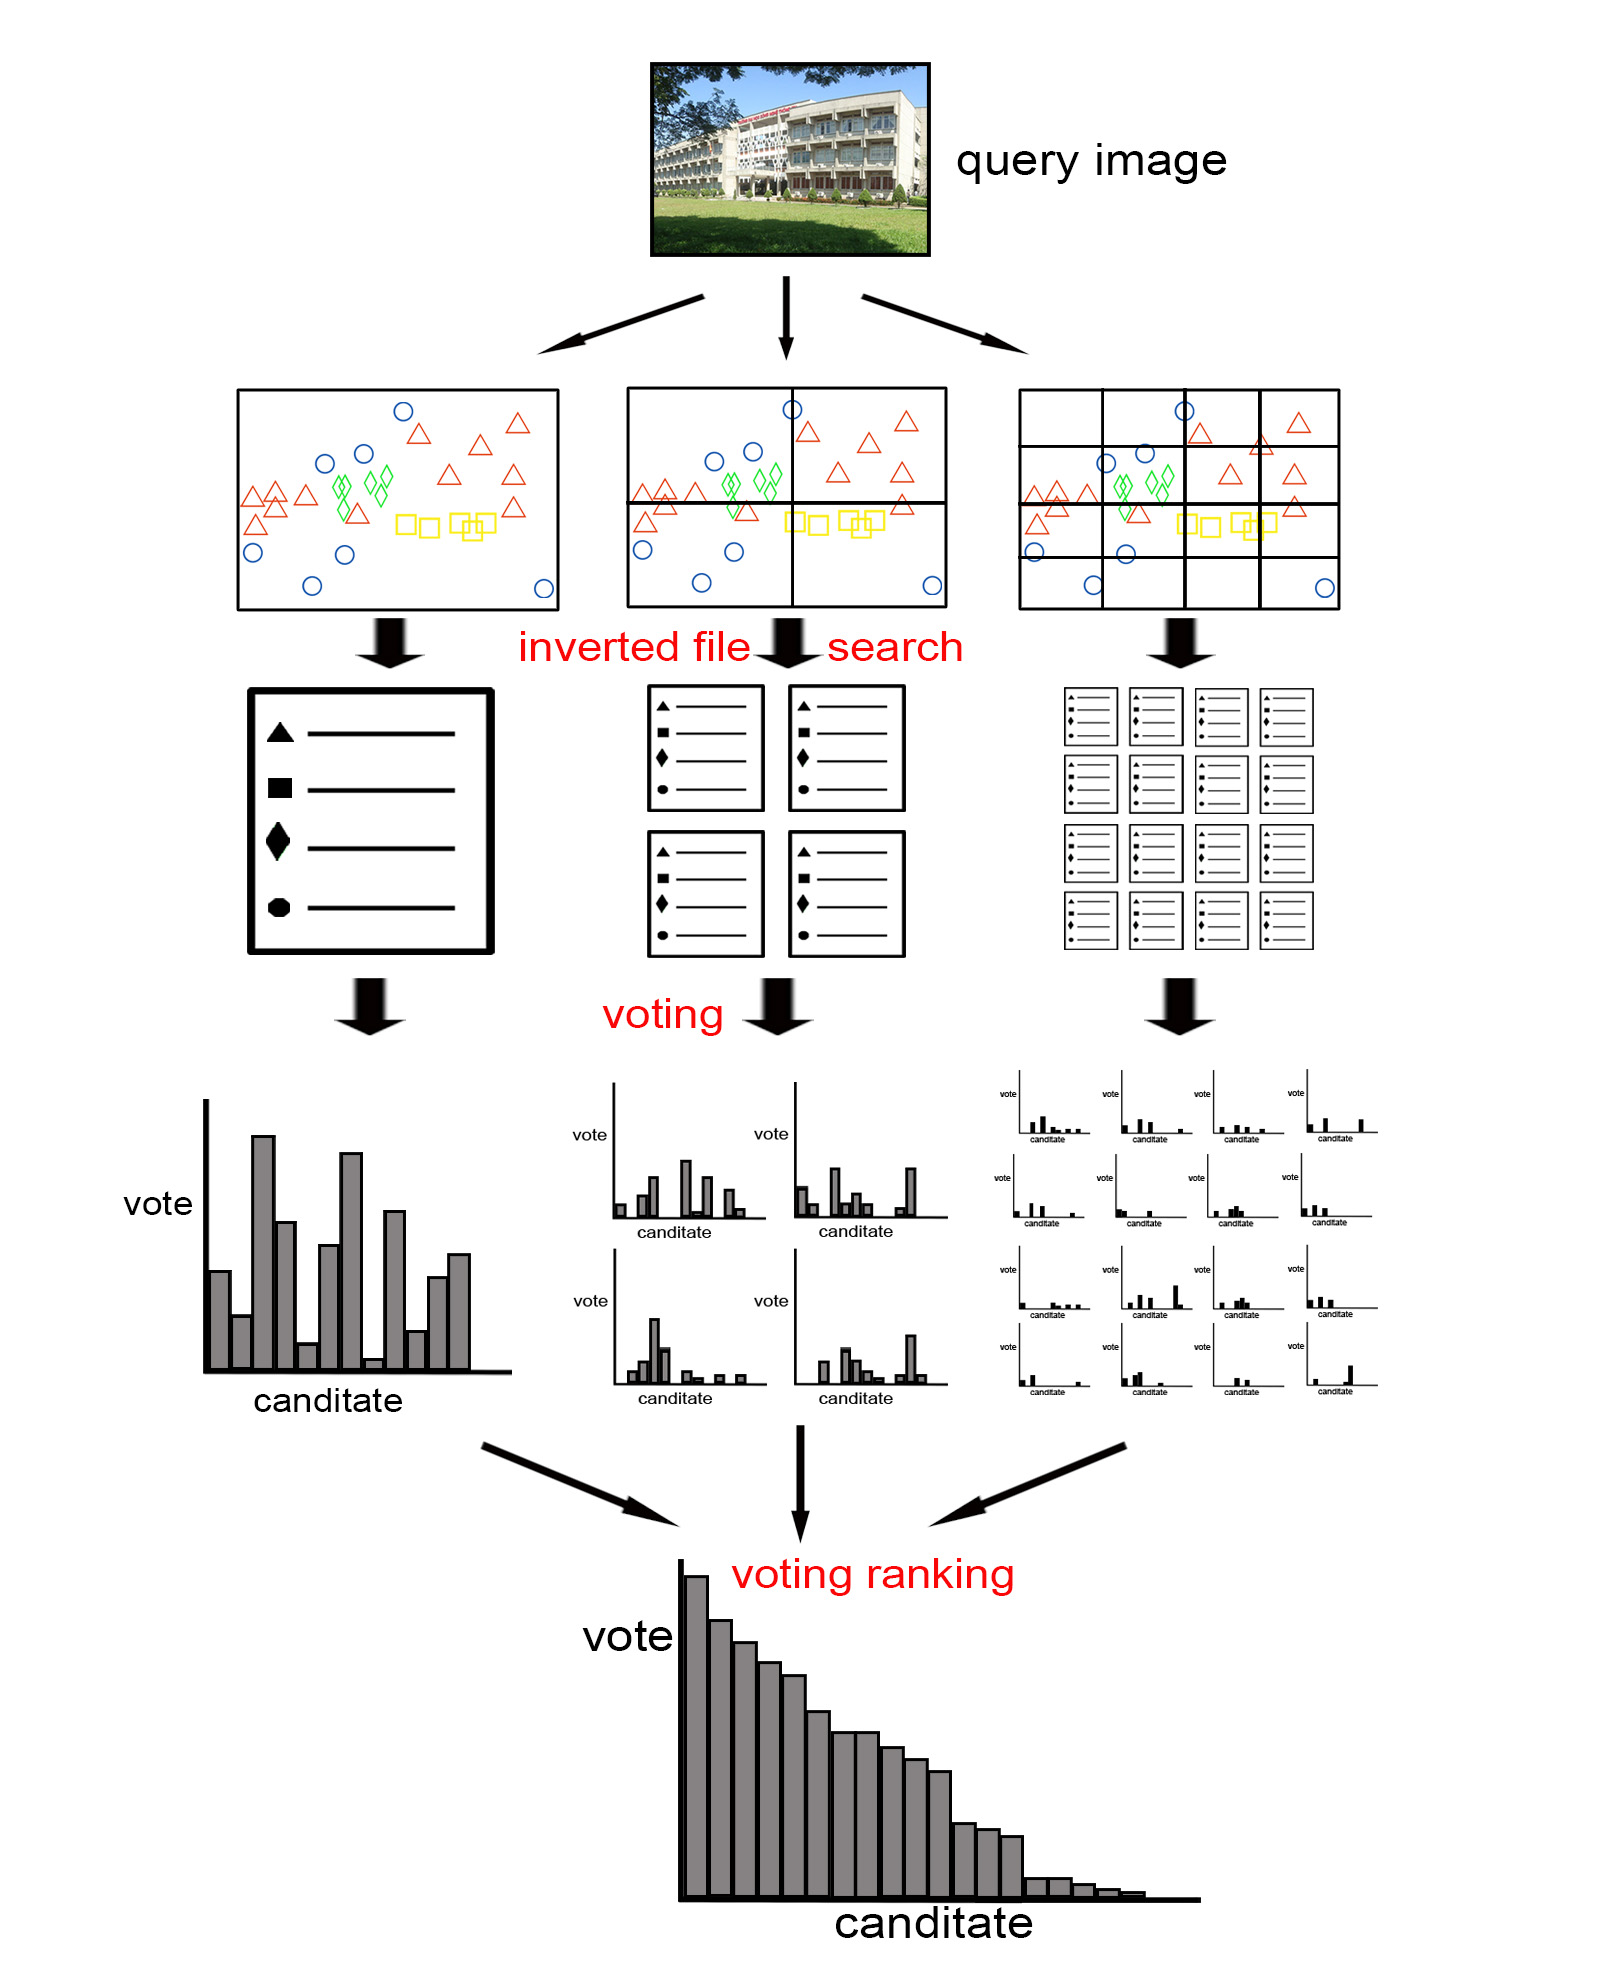
\includegraphics[scale=0.25]{queryProcess}
    \fi
    \caption[Quá trình truy vấn của phương pháp đề xuất]{Quá trình truy vấn của phương pháp đề xuất.}
    \label{FigQueryProcess}
  \end{center}
\end{figure}
